\documentclass[18pt, handout]{beamer}

\usetheme{metropolis}
\usefonttheme{professionalfonts}


%% "Patch" to keep the text widths' of Metropolis similar to that of Madrid.
%\setbeamersize{text margin left=15pt, text margin right=15pt}
%\makeatletter
%\setbeamertemplate{title page}{
%\centering
%  \begin{minipage}[b][\paperheight]{.9\textwidth}
%    \ifx\inserttitlegraphic\@empty\else\usebeamertemplate*{title graphic}\fi
%    \vfill%
%    \ifx\inserttitle\@empty\else\usebeamertemplate*{title}\fi
%    \ifx\insertsubtitle\@empty\else\usebeamertemplate*{subtitle}\fi
%    \usebeamertemplate*{title separator}
%    \ifx\beamer@shortauthor\@empty\else\usebeamertemplate*{author}\fi
%    \ifx\insertdate\@empty\else\usebeamertemplate*{date}\fi
%    \ifx\insertinstitute\@empty\else\usebeamertemplate*{institute}\fi
%    \vfill
%    \vspace*{1mm}
%  \end{minipage}
%}
%\makeatother

% Modify the text widths' of section title pages. See `beamerinnerthememetropolis.dtx`.
% `\paperheight` requires adjustment after modifying the frame content placement. Not sure why.
\makeatletter
\setbeamertemplate{section page}{
  \centering
  \begin{minipage}[c][.95\paperheight]{.9\textwidth}
    \raggedright
    \usebeamercolor[fg]{section title}
    \usebeamerfont{section title}
    \insertsectionhead\\[-1ex]
    \usebeamertemplate*{progress bar in section page}
    \par
    \ifx\insertsubsectionhead\@empty\else%
      \usebeamercolor[fg]{subsection title}%
      \usebeamerfont{subsection title}%
      \insertsubsectionhead
    \fi
  \end{minipage}
  \par
  \vspace{\baselineskip}
}
\makeatother

% Make frametitles larger and place closer to center. See `beamerinnerthememetropolis.dtx`.
\setbeamerfont{frametitle}{size=\Large}
\makeatletter
% Theme default adds paddings of 2.2ex to all the four sides of frame titles
\newlength{\metropolis@frametitle@toppadding}
\newlength{\metropolis@frametitle@bottompadding}
\setlength{\metropolis@frametitle@toppadding}{3.5ex} 
\setlength{\metropolis@frametitle@bottompadding}{0ex} 
\setlength{\metropolis@frametitle@padding}{4ex} % Horizontal padding to left
\renewcommand{\metropolis@frametitlestrut@start}{
  \rule{0pt}{\metropolis@frametitle@toppadding +%
    \totalheightof{%
      \ifcsdef{metropolis@frametitleformat}{\metropolis@frametitleformat X}{X}%
    }%
  }%
}
\newcommand*\getlength[1]{\number#1}
\renewcommand{\metropolis@frametitlestrut@end}{%
  \ifnum\getlength{\metropolis@frametitle@bottompadding}>0%
    \rule[-\metropolis@frametitle@bottompadding]{0pt}{\metropolis@frametitle@bottompadding}%
  \fi%
}
\makeatother

% Move up the frame content a bit. See:
% https://github.com/matze/mtheme/blob/master/source/beamerinnerthememetropolis.dtx#L509-L523
% https://tex.stackexchange.com/questions/247826/beamer-full-vertical-centering
\makeatletter
\define@key{beamerframe}{c}[true]{% centered
  \beamer@frametopskip=0pt plus 0.5fill\relax% Default is `1fill`
  \beamer@framebottomskip=0pt plus 1.5fill\relax%
  \beamer@frametopskipautobreak=0pt plus .4\paperheight\relax%
  \beamer@framebottomskipautobreak=0pt plus .6\paperheight\relax%
  \def\beamer@initfirstlineunskip{}%
}
\makeatother


%% Packages
\usepackage[english]{babel}
\usepackage{graphicx}
\usepackage{mathtools} % For \coloneqq (among others)
\usepackage{subcaption}
\usepackage{bm}
\usepackage{soul}
\usepackage{tikz}
\usetikzlibrary{bayesnet}
%\usepackage[normalem]{ulem}
%	\renewcommand{\ULthickness}{.6pt} % default is 0.4pt
%	\newcommand{\coloredUline}{\bgroup\markoverwith{\textcolor{lava}{\rule[-0.5ex]{2pt}{0.6pt}}}\ULon}
\usepackage{natbib}
	\bibliographystyle{abbrvnat}
	\setcitestyle{authoryear, open={(}, close={)}}
\usepackage{usebib}
\usepackage{bibentry} % For \nobibliography
\newbibfield{journal}
\bibinput{references}


%% Beamer options.
\setbeamercovered{dynamic}
\setbeamercovered{invisible}
\beamertemplatenavigationsymbolsempty
%\setbeamertemplate{caption}{unnumbered}
\setbeamertemplate{footline}{}
%\setbeameroption{show notes on second screen}

%% Customize styles inside itemize environments
%\settowidth{\leftmargini}{\usebeamertemplate{itemize item}}
%\addtolength{\leftmargini}{-1.2\labelsep}
\setbeamerfont{itemize/enumerate subbody}{size=\normalsize} %to set the body size
\setbeamertemplate{itemize subitem}{\normalsize\raise1.25pt\hbox{\donotcoloroutermaths$\blacktriangleright$}}  % to set the symbol size

%% Custom environments
\newcommand{\defineTightSpacing}{%
	\setlength{\abovedisplayskip}{.25\baselineskip}%
	\setlength{\belowdisplayskip}{.25\baselineskip}%
}
\newenvironment{tightEquation}{%
	\defineTightSpacing%
	\begin{equation}
}{
	\end{equation} \ignorespacesafterend
}
\makeatletter
\newenvironment{tightEquation*}{%
	\defineTightSpacing%
	\begin{equation*}
}{
	\end{equation*} \ignorespacesafterend
}
\newcommand{\defineWithinItemizeSpacing}{%
	\setlength{\abovedisplayskip}{.3\baselineskip}%
	\setlength{\belowdisplayskip}{.3\baselineskip}%
}
\newenvironment{itemizedEquation}{%
	\defineWithinItemizeSpacing%
	\begin{equation}
}{
	\end{equation} \ignorespacesafterend
}
\makeatletter
\newenvironment{itemizedEquation*}{%
	\defineWithinItemizeSpacing%
	\begin{equation*}
}{
	\end{equation*} \ignorespacesafterend
}
\newenvironment{indented}[1][3]{%
	\hfill \begin{minipage}{\dimexpr\textwidth-#1ex} 
	}{
	\end{minipage}
}
\newenvironment{wideitemize}{%
  \begin{itemize}
  \addtolength\itemsep{.4\baselineskip}
}{
  \end{itemize}
}
\newenvironment{tightItemize}[1][]{%
  \vspace{-.3\baselineskip}%
  \begin{itemize}[#1]
  \addtolength\itemsep{-.1\baselineskip}
}{
  \end{itemize}
}
\newenvironment{tightEnumerate}[1][1.]{%
  \vspace{-.3\baselineskip}%
  \begin{enumerate}[#1]
  \addtolength\itemsep{-.1\baselineskip}
}{
  \end{enumerate}
}

%% Color definitions
\definecolor{turquoise}{rgb}{0.19, 0.84, 0.78}
\definecolor{mediumturquoise}{rgb}{0.28, 0.82, 0.8}
\definecolor{lava}{rgb}{0.81, 0.06, 0.13}
\colorlet{linkColor}{mediumturquoise}
\colorlet{highlightedTextColor}{lava}

%% Set the color theme of the presentation
\definecolor{jhuBlue}{RGB}{0, 45, 114} % "Heritage" blue; https://brand.jhu.edu/color/
\definecolor{jhuSpiritBlue}{RGB}{114, 172, 229} % lighter blue
\colorlet{themecolor}{jhuBlue}
\colorlet{bgcolor}{themecolor}
\colorlet{textcolor}{white}
\usecolortheme[named=themecolor]{structure}
%\setbeamercolor{titlelike}{fg=black}
\setbeamercolor{frametitle}{fg=themecolor, bg=white}
\setbeamercolor{section in head/foot}{fg=textcolor}
\setbeamercolor{background canvas}{bg=white}
%\colorlet{toccolor}{black}
%\setbeamercolor{section in toc}{fg=toccolor}
\setbeamercolor{block title}{bg=themecolor!75!gray!25}
\setbeamercolor{block body}{bg=themecolor!75!gray!5}


% Macros

%% Utility macros
\newcommand{\noteBullet}{\hspace*{.75em}\textcolor{themecolor}{$\blacktriangleright$}\ }
\renewcommand{\textsc}[1]{{\small \MakeUppercase{#1}}}

%% General math macros
\newcommand{\given}{\thinnerspace | \thinnerspace}
\newcommand{\spacedColon}{\mkern .5mu : \mkern 1mu}
\newcommand{\spacedEq}{\mkern 1mu = \mkern 1.5mu}
\newcommand{\divby}{\thinnerspace /}
\newcommand{\defeq}{\vcentcolon =} % `\coloneqq` and `\vcentcolon` requires the `mathtools` package: https://tex.stackexchange.com/questions/194344/symbol-for-definition
\newcommand{\diff}{\operatorname{\mathrm{d}}\!{}}
\newcommand{\sign}{\mathrm{sign}}
\newcommand{\diag}{\mathrm{diag}}
\newcommand{\medcap}{\mathbin{\mathsmaller{\bigcap}}}
\DeclareMathOperator*{\argmin}{argmin}
\DeclareMathOperator*{\argmax}{argmax}
\newcommand{\elemwiseProd}{\odot}
\renewcommand{\complement}{{\raisebox{1.5pt}{\scriptsize $\mathsf{c}$}}}
\newcommand{\transpose}{\text{\raisebox{.5ex}{$\intercal$}}}
\newcommand{\higherTranspose}{\text{\raisebox{.9ex}{$\intercal$}}}
\newcommand{\lowerscript}[1]{\raisebox{-2pt}{\scriptsize $#1$}}
\newcommand{\yesnumber}{\addtocounter{equation}{1}\tag{\theequation}}
\newcommand{\thinnerspace}{\mskip.5\thinmuskip}
\newcommand{\thinnestspace}{\mskip.25\thinmuskip}
\newcommand{\negthinnerspace}{\mskip-.5\thinmuskip}
\newcommand{\spaceBeforePartial}{\mskip\thinmuskip}
\newcommand{\scriptsumi}{{\scriptsize \sum_i}} % Suscript needs to be within bracket, hence the hard coding

%%% Define a larger "hat" of fixed width: https://tex.stackexchange.com/questions/20473/how-can-i-manually-choose-the-size-of-a-wide-accent-math-mode/20477#20477
\DeclareMathSymbol{\widehatsym}{\mathord}{largesymbols}{"62}
\newcommand{\lowerwidehatsym}{\text{\smash{\raisebox{-1.3ex}{$\widehatsym$}}}}
\newcommand\fixedwidehat[1]{%
  \mathchoice
    {\accentset{\displaystyle\lowerwidehatsym}{#1}}
    {\accentset{\textstyle\lowerwidehatsym}{#1}}
    {\accentset{\scriptstyle\lowerwidehatsym}{#1}}
    {\accentset{\scriptscriptstyle\lowerwidehatsym}{#1}}
}

%% Probability / statistics macros
\newcommand{\probability}{\mathbb{P}}
\newcommand{\expectation}{\mathbb{E}}
\newcommand{\variance}{\mathrm{Var}}
\DeclareMathOperator*{\covariance}{Cov}
\newcommand{\indicator}{\mathds{1}}
\newcommand{\eqDistribution}{\mathrel{\raisebox{-.2ex}{$\overset{\scalebox{.6}{$\, d$}}{=}$}}}
\newcommand{\iidSim}{\mathrel{\raisebox{-.3ex}{$\overset{\text{i.i.d.}}{\sim}$}}}
\newcommand{\unifDist}{\mathrm{Unif}}
\newcommand{\normalDist}{\mathcal{N}}
\newcommand{\betaDist}{\mathrm{Beta}}
\newcommand{\gammaDist}{\mathrm{Gamma}}
\newcommand{\mle}[1]{\widehat{#1}_{\textrm{mle}}}
\newcommand{\map}[1]{\widehat{#1}_{\textrm{map}}}
\newcommand{\empiricalVar}{\widehat{\variance}}
\newcommand{\kldivergence}{D_{\mathrm{KL}}}
\newcommand{\truthSub}{\mathrm{tru}}

%% Variable macros / Aliases
\newcommand{\nPred}{p}
\newcommand{\nObs}{n}
\newcommand{\density}{\pi}
\newcommand{\likelihood}{L}
\newcommand{\infoMat}{\mathcal{I}}
\newcommand{\by}{\bm{y}}
\newcommand{\bx}{\bm{x}}
\newcommand{\bX}{\bm{X}}
\newcommand{\vecRv}{\mathbf{X}}
\newcommand{\bmu}{\bm{\mu}}
\newcommand{\bbeta}{\bm{\beta}}
\newcommand{\btheta}{\bm{\theta}}
\newcommand{\Id}{\bm{I}}
\newcommand{\bPhi}{\bm{\Phi}}
\newcommand{\bSigma}{\bm{\Sigma}}

%% For cross-validation 
\newcommand{\loss}{\mathcal{L}}
\newcommand{\score}{\mathcal{S}}
\newcommand{\modelSymbol}{\mathcal{M}}
\newcommand{\permutation}{\rho}
\newcommand{\trainingSize}{m}
\newcommand{\testSampleIndex}{i}
\newcommand{\testOutcome}{y_{\permutation(\testSampleIndex)}} % 
\newcommand{\testOutcomePredicted}{\widehat{y}_{\permutation(\testSampleIndex)}^{\, \trainingSize}} 
	% Other candidates previously explored: 1) $\by^\trainingSize_\permutation$, 2) $\widehat{y}_{\permutation}^{\, \trainingSize}\mkern-1mu\big( \testPred \big)$
\newcommand{\testPred}{\bx_{\permutation(\testSampleIndex)}}
\newcommand{\trainOutcome}{y_{\permutation(1 \spacedColon \trainingSize)}}
\newcommand{\trainPred}{\bx_{\permutation(1 \spacedColon \trainingSize)}}


\title{%
	\centering Controlling model complexity: Bayesian interpretation of regularization/shrinkage%
}
\author{%
	Aki Nishimura\\
	Department of Biostatistics%
}
%\institute[]{}
\date{}

\titlegraphic{%
	\begin{picture}(0,0)
		% Try coordinate (155, -150) for a one-line title, (165, -160) if two-lines, and (155, -172) if three-lines
		\put(165, -160){\makebox(0,0)[lb]{
\includegraphics[width=.45\textwidth]{jhsph_biostat_logo}}}
	\end{picture}%
}

\begin{document}

\maketitle


\begin{frame}
\frametitle{Rise of shrinkage estimation}
One measure of a statistical estimator's quality is its {\small MSE}:
\begin{tightEquation*}
\operatorname{MSE}_{\btheta_\truthSub\!}(\widehat{\btheta})
	= \expectation \thinnerspace \big\| \widehat{\btheta} - \btheta_\truthSub \big\|^2
	= \expectation_{\thinnerspace \by \thinnerspace \sim \thinnerspace  \likelihood(\thinnerspace \cdot \given \btheta_\truthSub)\!}\!\left[
		\big\| \widehat{\btheta}(\by) - \btheta_\truthSub \big\|^2
	\right].
\end{tightEquation*}

M{\small SE} in particular illustrates a bias-variance trade-off in estimation:
\begin{tightEquation*}
\expectation \thinnerspace \big\| \widehat{\btheta} - \btheta_\truthSub \big\|^2
	= \big\| \expectation\thinnerspace\widehat{\btheta} - \btheta_\truthSub \big\|^2
	+ \variance(\widehat{\btheta}).
\end{tightEquation*}

\cite{stein1956inadmissibility} demonstrates a potential benefit of bias --- 
he consider a problem of estimating unknown means under the model
\begin{tightEquation*}
y_i \given \mu_i
	\sim \normalDist(\mu_i, \sigma^2)
	\ \text{ for } \, i = 1, \ldots, n 
	% Note: $\phi$ is assumed fixed for simplicity.
\end{tightEquation*}
and constructs an estimator that \textit{always} beats $\mle{\bmu} = \by$ in {\small MSE}.
\end{frame}


\begin{frame}
\frametitle{Rise of shrinkage estimation}
\begin{theorem}\upshape
The {\small MLE} is \textit{inadmissible} in $n > 2$, with the James-Stein estimator 
\begin{tightEquation*}
\widehat{\bmu}_{\mathrm{JS}}(\by) = \left( 1 - \frac{(n - 2) \sigma^2}{\| \by \|^2} \right) \by
\end{tightEquation*}
having a lower {\small MSE} than $\mle{\bmu} = \by$ for \textit{any} underlying $\bmu_\truthSub$.
\end{theorem}
\vspace*{-.2\baselineskip}
JS estimator is an example of \textit{shrinkage estimators}, taking a form $\widehat{\mu_i} = c_i \thinnerspace y_i$ for $ c_i \in (0, 1)$ that biases the estimate towards 0.

\smallskip
Technically, ``shrinkage'' in $\widehat{\bmu}_{\mathrm{JS}}$ is only true with high probability: 
$\expectation \thinnerspace \| \by \|^2 
%	= \expectation\!\left[ \expectation[\| \by \|^2 \given \bmu] \right] 
	= \| \bmu \|^2  + n \sigma^2$,
so we expect $(n - 2) \sigma^2 / \| \by \|^2 < 1$.

\smallskip
Better yet, the following modification improves on $\widehat{\bmu}_{\mathrm{JS}}$:
\begin{tightEquation*}
\widehat{\bmu}_{\mathrm{B}}(\by) = \left[ 1 - \frac{(n - 2) \sigma^2}{\| \by \|^2} \right]^+ \! \by.
	% Note: Subscript "B" for Baranchik (1970), "A family of minimax estimators of the mean of a multivariate normal distribution."
\end{tightEquation*}
\end{frame}


\begin{frame}
\frametitle{M{\normalsize SE} of Gaussian mean estimator}
By routine algebra,
\begin{equation*} \defineTightSpacing%
\| \widehat{\bmu} - \bmu \|^2
	= - \| \by - \bmu \|^2 + \| \by - \widehat{\bmu} \|^2 
		+ 2 \left\langle \by - \bmu, \widehat{\bmu} - \bmu \right\rangle.
\end{equation*}
Taking expectations, we have
\begin{equation*} \defineTightSpacing%
\expectation \| \widehat{\bmu} - \bmu \|^2
	= - n \sigma^2 + \expectation \| \by - \widehat{\bmu} \|^2 
%		+ 2 \thinnerspace {\textstyle \sum_i} \covariance(y_i, \widehat{\mu}_i).
		+ 2 \thinnerspace {\textstyle \sum_i} \thinnerspace \expectation[ (\widehat{\mu}_i - \mu_i) (y_i - \mu_i) ].
\end{equation*}

We now invoke \textit{Stein's lemma}: if $\mathbf{Y} \sim \normalDist(\bmu, \bSigma)$ and $f: \mathbb{R}^n \to \mathbb{R}$, 
\begin{equation*} \defineTightSpacing%
\expectation[ f(\mathbf{Y}) (\mathbf{Y} - \bmu) ] = \bSigma \, \expectation[ \nabla \negthinnerspace f(\mathbf{Y})].
\end{equation*}
Applying the lemma to $f(\by) = \widehat{\mu}_i(\by) - \mu_i$ yields
\begin{equation*} \defineTightSpacing%
\expectation[ (\widehat{\mu}_i - \mu_i) (\by - \bmu) ] 
	= \sigma^2 \thinnerspace \expectation[ \nabla \widehat{\mu}_i(\by)].
\end{equation*}

Plugging this into the earlier equality:
\begin{equation*} \defineTightSpacing%
\expectation \| \widehat{\bmu} - \bmu \|^2
	= - n \sigma^2 + \expectation \| \by - \widehat{\bmu} \|^2 
%		+ 2 \thinnerspace {\textstyle \sum_i} \covariance(y_i, \widehat{\mu}_i).
		+ 2 \sigma^2 \thinnerspace {\textstyle \sum_i} \thinnerspace \expectation\!\left[ \frac{\partial \widehat{\mu}_i}{\partial y_i}  \right].
\end{equation*}
	% Note: SURE's value lies in the fact that the right-hand side does not depend on the true, unknown $\bmu$. So you can estimate MSE without knowing $\bmu$ and, for example, try to minimize it.
\end{frame}


\begin{frame}
\frametitle{M{\normalsize SE} of Gaussian mean estimator}
What we've derived, essentially, is \textit{Stein's unbiased risk estimator}:
\begin{equation*} \defineTightSpacing%
\widehat{\operatorname{MSE}}
	= - n \sigma^2 +  \| \by - \widehat{\bmu} \|^2 
		+ 2 \sigma^2 \thinnerspace {\textstyle \sum_i} \frac{\partial \widehat{\mu}_i}{\partial y_i}.
\end{equation*}
\vspace*{-.7\baselineskip}

We now calculate \textsc{SURE} for $\, \widehat{\bmu}_{\mathrm{JS}}(\by) = \left( 1 - \frac{(n - 2) \sigma^2}{\| \by \|^2} \right) \! \by$. 
Note
\begin{equation*} \defineTightSpacing%
\| \by - \widehat{\bmu}_{\mathrm{JS}} \|^2 
	= \left\| \frac{(n - 2) \sigma^2}{\| \by \|^2} \by \thinnerspace \right\|^2 
	= \frac{(n - 2)^2 \sigma^4}{\| \by \|^2},
%+ 2 \sigma^2 \thinnerspace {\textstyle \sum_i} \frac{\partial \widehat{\mu}_i}{\partial y_i}.
\end{equation*}
and
\begin{equation*} \defineTightSpacing%
\frac{\partial \widehat{\mu}_{\mathrm{JS}, i}}{\partial y_i}
	= \left( 1 - \frac{(n - 2) \sigma^2}{\| \by \|^2} \right) - (n - 2) \sigma^2 y_i \thinnerspace \frac{\partial}{\partial y_i} \frac{\!\!1}{\| \by \|^2}.
\end{equation*}

\smallskip
Since $\frac{\partial}{\partial y_i} \frac{\!\!1}{\| \by \|^2} = - \frac{\!\!2 y_i}{\| \by \|^4}$ and $\sum_i  y_i \thinnerspace \frac{\partial}{\partial y_i} \frac{\!\!1}{\| \by \|^2} = - \frac{\!\!2}{\| \by \|^2}$ , we have
\begin{equation*} \defineTightSpacing%
{\textstyle \sum_i} \frac{\partial \widehat{\mu}_{\mathrm{JS}, i}}{\partial y_i}
	= n \left( 1 - \frac{(n - 2) \sigma^2}{\| \by \|^2} \right) + \frac{2 (n - 2) \sigma^2}{\| \by \|^2} % 2 (n - 2) \sigma^2\frac{\!\!1}{\| \by \|^2}
	= n - \frac{(n - 2)^2 \sigma^2}{\| \by \|^2}.
\end{equation*}
\end{frame}


\begin{frame}
\frametitle{M{\normalsize SE} of Gaussian mean estimator}
So \textsc{SURE} for $\widehat{\bmu}_{\mathrm{JS}}$ is given by
\begin{equation*} \defineTightSpacing%
\begin{aligned}
\widehat{\operatorname{MSE}}_{\mathrm{JS}}
	&= - n \sigma^2 
		+ \frac{(n - 2)^2 \sigma^4}{\| \by \|^2}
		+ 2 n \sigma^2 
		- 2 \frac{(n - 2)^2 \sigma^4}{\| \by \|^2} \\
	&= n \sigma^2 - \frac{(n - 2)^2 \sigma^4}{\| \by \|^2}.
\end{aligned}
\end{equation*}

Taking expectations, we obtain
\begin{equation*} \defineTightSpacing%
\expectation \| \widehat{\bmu}_{\mathrm{JS}} - \bmu \|^2 
	= n \sigma^2  - (n - 2)^2 \sigma^4 \thinnerspace \expectation\!\left[ \frac{\!\!1}{\| \by \|^2} \right] 
%	\leq n \sigma^2
	\leq \expectation \| \by - \bmu \|^2.
\end{equation*}
\end{frame}

\begin{frame}
\frametitle{M{\normalsize SE} of Gaussian mean estimator}
This reduction in \textsc{MSE} can be substantial.
For large $n$, we have
\begin{equation*} \defineTightSpacing%
\frac{1}{n} \| \by \|^2 \approx \frac{1}{n} \| \bmu \|^2 + \sigma^2.
\end{equation*}

Taking expectations, we obtain
\begin{equation*} \defineTightSpacing%
\begin{aligned}
\expectation \| \widehat{\bmu}_{\mathrm{JS}} - \bmu \|^2 
	&= n \sigma^2  - (n - 2)^2 \sigma^4 \thinnerspace \expectation\!\left[ \frac{\!\!1}{\| \by \|^2} \right] \\
	&= n \sigma^2 \left(
		1 - \frac{(n - 2)^2}{n^2} \expectation\!\left[ \frac{n \sigma^2}{\| \by \|^2} \right] 
	\right) \\
	&\sim n \sigma^2 \left(
		1 - \frac{\sigma^2}{\sigma^2 + n^{-1} \| \bmu \|^2} 
	\right)
	\ \text{ as } \, n \to \infty.
\end{aligned}
\end{equation*}

So the reduction is roughly determined by noise vs.\ signal size (i.e.\ $\sigma^2$ vs.\ $n^{-1} \| \bmu \|^2$);
e.g.  $\sigma^2 \approx n^{-1} \| \bmu \|^2$ leads to 50\% (!) reduction. 
\end{frame}


\begin{frame}
\frametitle{Shrinkage in action: Famous batting ave example}
% Note: How Efron and Morris dealt with unequal variances is discussed here: https://stats.stackexchange.com/questions/119786/james-stein-estimator-with-unequal-variances.
\begin{figure}
\centering
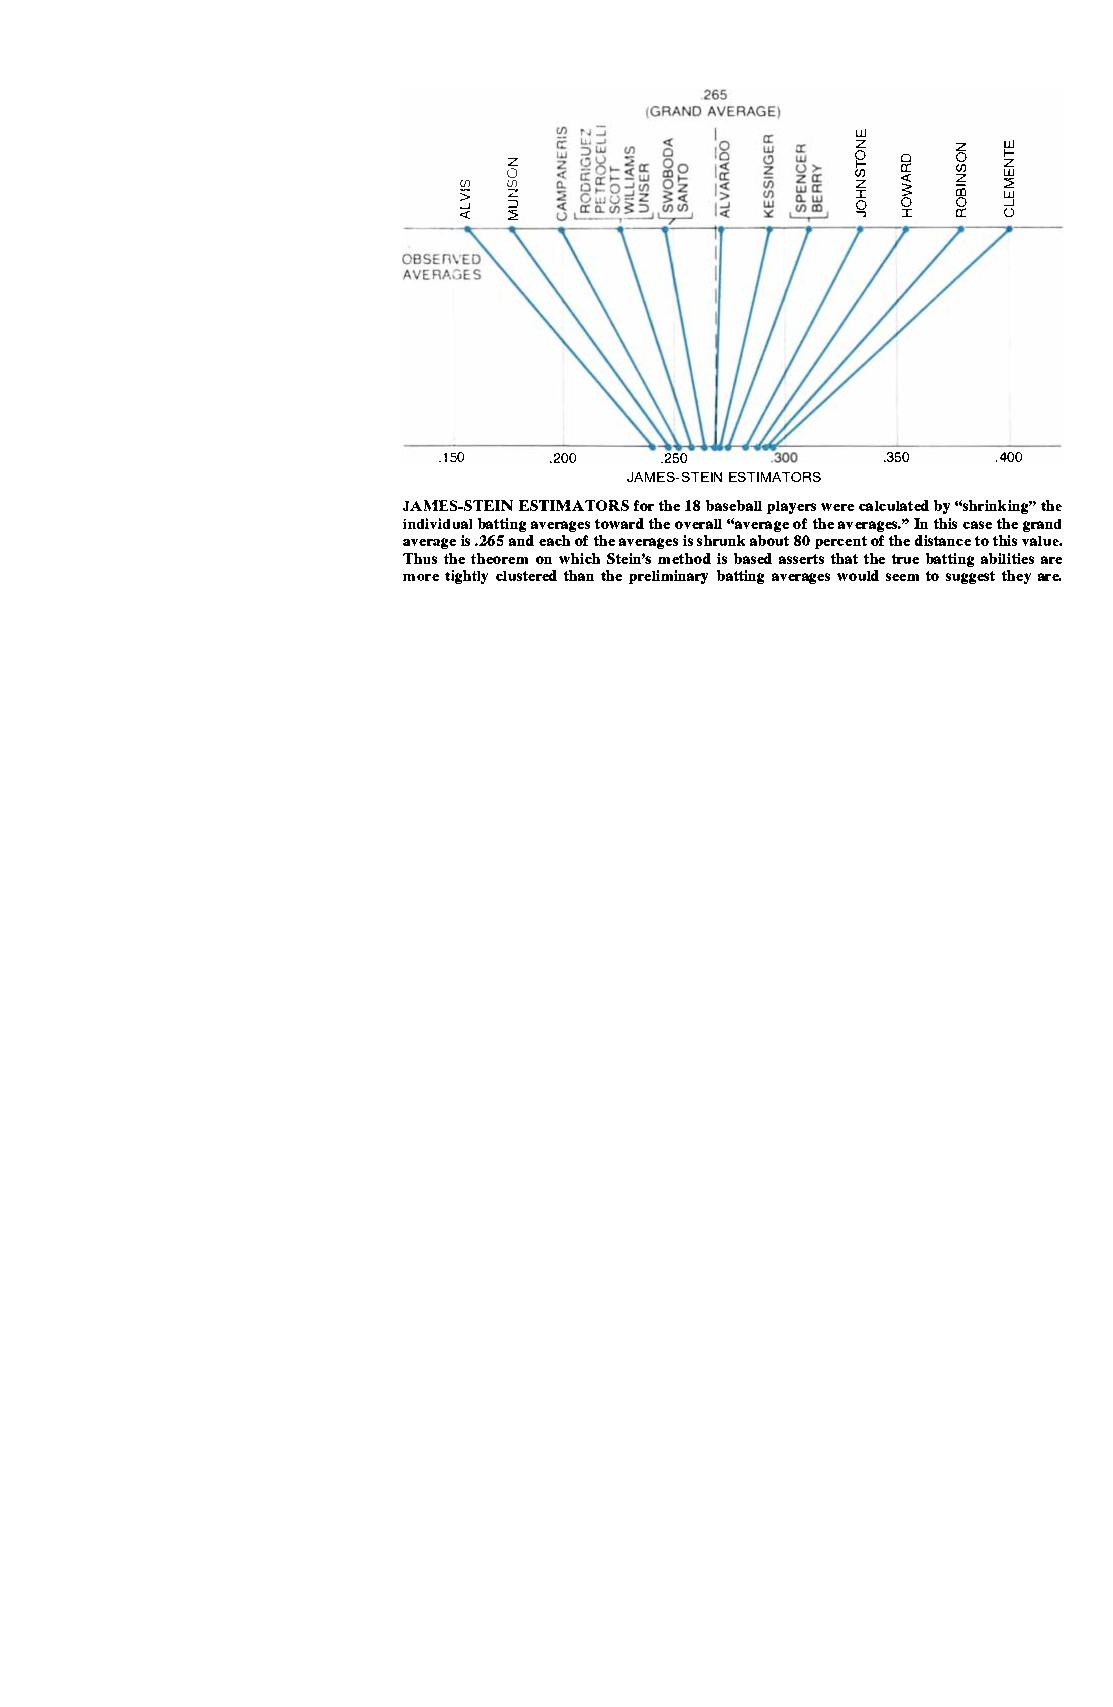
\includegraphics[width=.75\linewidth]{Figure/batting_ave_example_scientific_american}
\caption*{\textcolor{themecolor}{\textbf{Figure:}}
	Predicting the 1970 season's performance from first 45 at bat\\ \hfill \citep{efron1977stein_sci_american}.%
}%
\end{figure}
\end{frame}


\begin{frame}
\frametitle{Shrinkage in action: Famous batting ave example}
\vspace*{-.5\baselineskip}
\begin{figure}
\centering
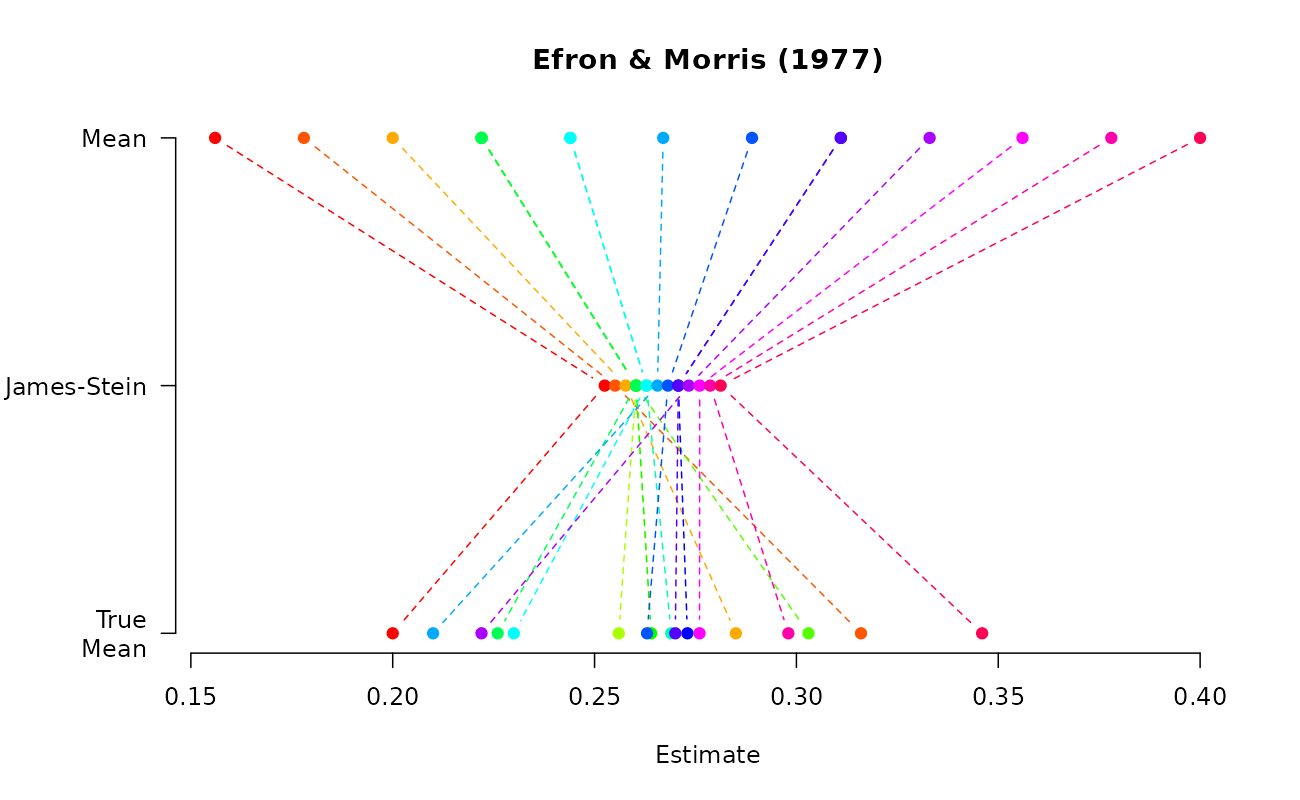
\includegraphics[width=.9\linewidth]{Figure/batting_ave_example_viz}
% Credit: https://r.tquant.eu/UvA/JamesSteinEstimator/
\vspace*{-.5\baselineskip}
\caption*{\textcolor{themecolor}{\textbf{Figure:}}
	Comparing JS estimates and observed season performances.%
}%
\end{figure}

\vspace*{-.8\baselineskip}
\textbf{Note:} The large amount of shrinkage is a known drawback.
\end{frame}


\begin{frame}
\frametitle{Shrinkage in action:  Toxoplasmosis example}
\begin{figure}
\centering
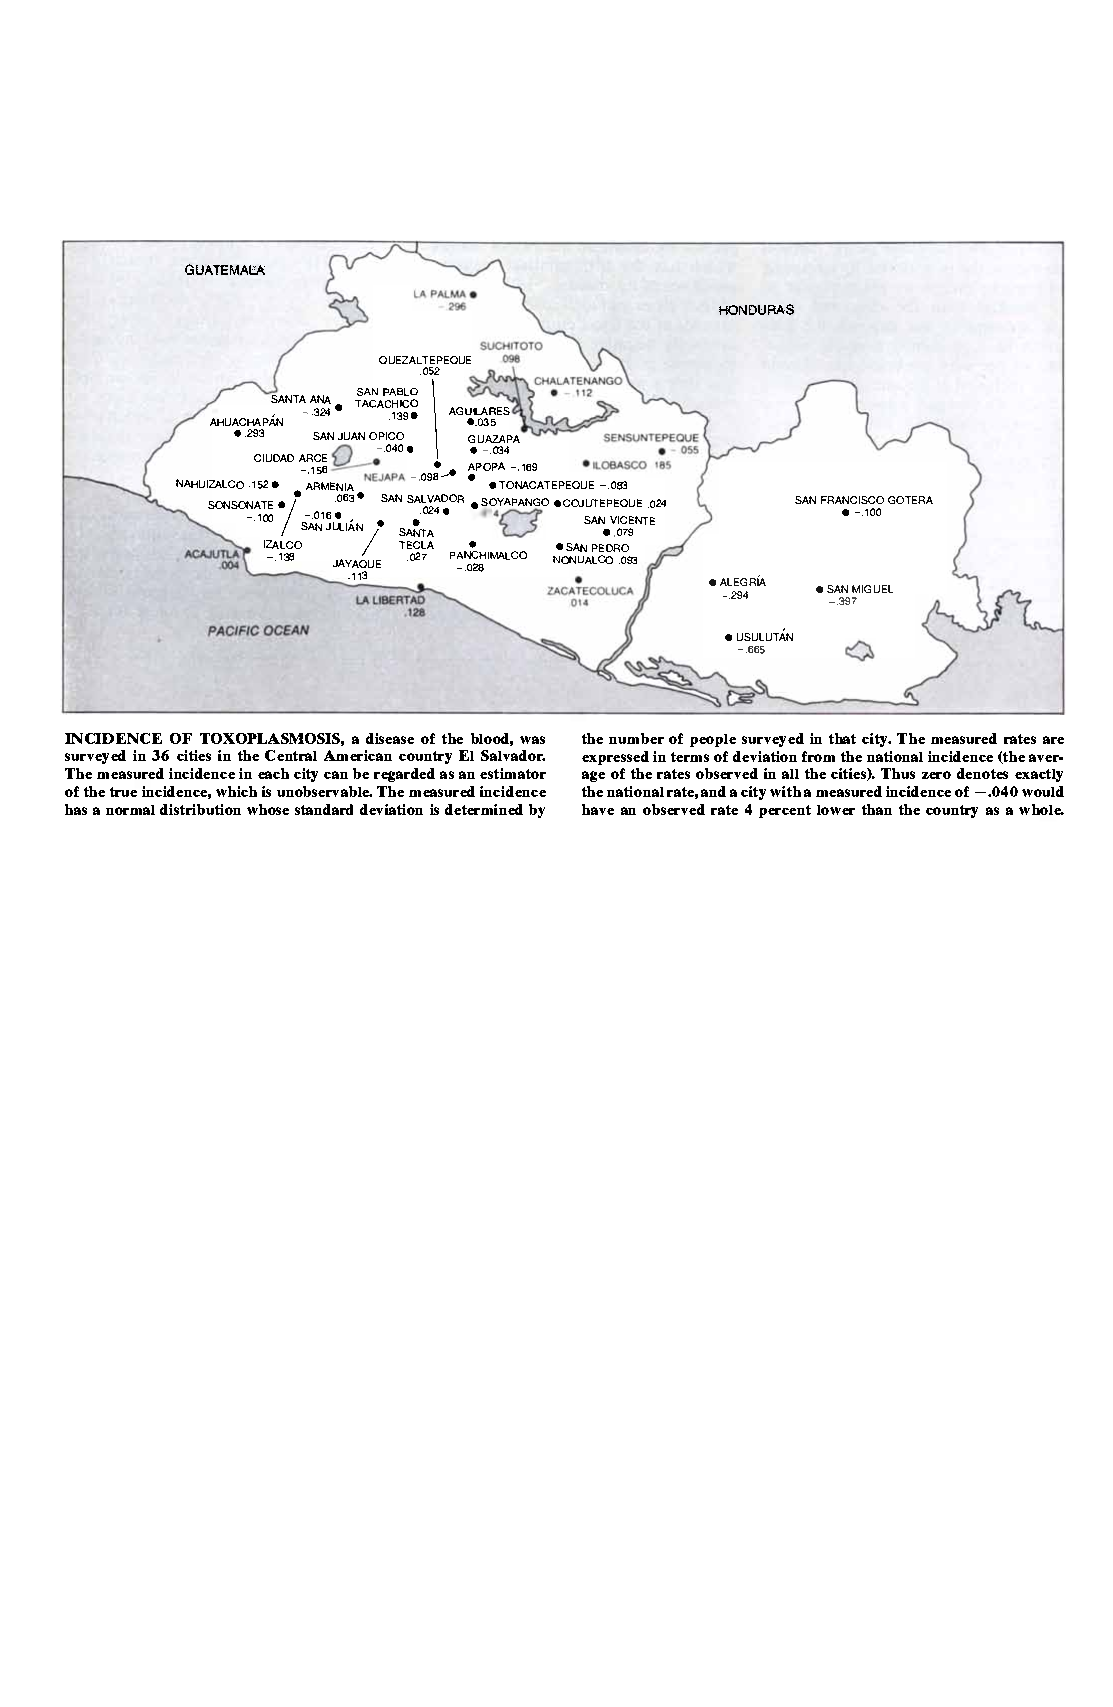
\includegraphics[width=\linewidth]{Figure/toxoplasmosis_example_map_scientific_american}
\end{figure}
\end{frame}


\begin{frame}
\frametitle{Shrinkage in action:  Toxoplasmosis example}
\begin{figure}
\centering
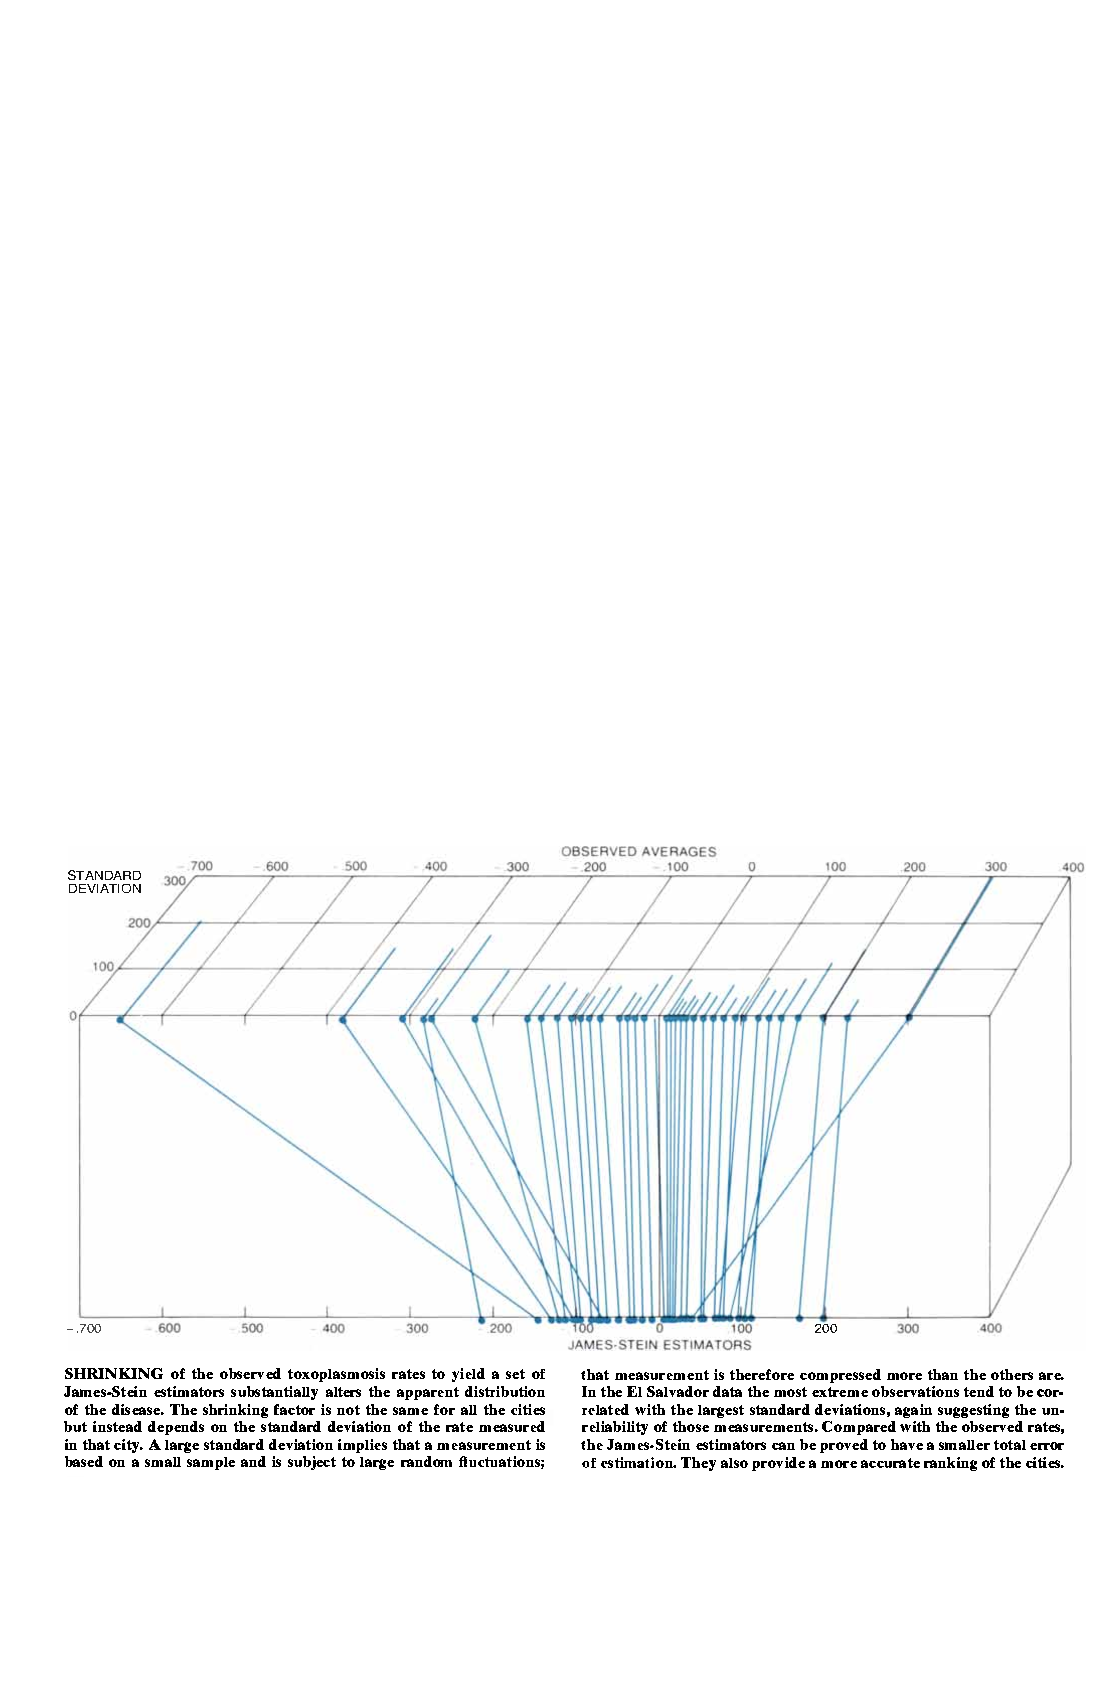
\includegraphics[width=\linewidth]{Figure/toxoplasmosis_example_scientific_american}
\end{figure}
\end{frame}


\begin{frame}
\frametitle{Shrinkage through Bayes lens}
Let's now consider estimating $\mu_i$'s through a random effect model
\begin{tightEquation*}
y_i \given \mu_i
	\sim \normalDist(\mu_i, \phi^{-1}\! = \sigma^2), \ \,
\mu_i \given \phi_{\textrm{grp}} 
	\sim \normalDist(0, \phi_{\textrm{grp}}^{-1}\! = \sigma_{\textrm{grp}}^2).
\end{tightEquation*}

The posterior, 
$\mu_i \given y_i, \phi_{\textrm{grp}} \sim \normalDist\!\left(
	\frac{\phi}{\phi + \phi_{\textrm{grp}}} y_i, \thinnerspace
	\frac{1}{\phi + \phi_{\textrm{grp}}}
\right)$,
gives rise to 
\begin{tightEquation*}
\hat{\bmu}_{\textrm{bayes}}
	= \left( 1 - \frac{\phi_{\mathrm{grp}}}{\phi + \phi_{\mathrm{grp}}} \right) \by
	= \left( 1 - \frac{\sigma^2}{\sigma^2 + \sigma^2_{\mathrm{grp}}} \right) \by.
\end{tightEquation*}

\smallskip
% Note $\thinnerspace \expectation \| \by \|^2 = n (\sigma^2 + \sigma_{\mathrm{grp}}^2)$ under this model, so $\frac{\sigma^2}{\sigma^2 + \sigma^2_{\mathrm{grp}}} \approx \frac{n \sigma^2}{\| \by \|^2}$.

Assuming the model to be correct, this is the Bayes estimator we would use if we knew $\phi_{\mathrm{grp}}$.
\end{frame}


\begin{frame}
\frametitle{Shrinkage through Bayes lens}
What $\phi_{\mathrm{grp}}$ should we use for an appropriate amount of shrinkage?

\smallskip
The fully Bayesian way is to place a prior on $\phi_{\mathrm{grp}}$ and estimate it along with $\mu_i$'s, but here we pursue quasi-Bayes, freq alternatives.

\smallskip
One method estimates the desired shrinkage factor $\frac{\sigma^2}{\sigma^2 + \sigma^2_{\mathrm{grp}}}$ from the observed $\by$.
To this end, we note $y_i \sim \normalDist(0, \sigma^2 + \sigma_{\mathrm{grp}^2})$ and
\begin{tightEquation*}
\| \by \|^2
	= \textstyle \sum_i y_i^2 
	\sim (\sigma^2 + \sigma_{\mathrm{grp}}^2) \thinnerspace \chi_n^2.
\end{tightEquation*}

This means $\expectation\!\left[ \frac{\!1}{\| \by \|^2} \right] = \frac{1}{(n - 2) (\sigma^2 + \sigma_{\mathrm{grp}}^2)}$ and therefore
\begin{tightEquation*}
\expectation\!\left[ \frac{(n - 2) \sigma^2}{\| \by \|^2} \right]
	= \frac{\sigma^2}{\sigma^2 + \sigma_{\mathrm{grp}}^2}. \ \text{ (!)}
\end{tightEquation*}

% Note: chi-square(df = \nu) ~ Gamma(shape = \nu / 2, rate = 1 / 2) -> 1 / chi-square(df = \nu) ~ InverseGamma(shape = \nu / 2, scale = 2)
\end{frame}


\begin{frame}
\frametitle{Shrinkage through Bayes lens}
Another method is more in line, while not fully so, with Bayesian thinking and considers maximizing the \textit{marginal likelihood}:
\begin{tightEquation*}
\likelihood(\by \given \phi_{\mathrm{grp}})
	= \int \likelihood(\by \given \bmu, \phi_{\mathrm{grp}}) \thinnerspace \density(\bmu \given \phi_{\mathrm{grp}}) \diff  \bmu.
\end{tightEquation*}

Since $y_i \sim \normalDist(0, \phi_{\mathrm{mg}}^{-1})$ for $\phi_{\mathrm{mg}}^{-1} = \phi^{-1} + \phi_{\mathrm{grp}}^{-1}$, we have
\begin{tightEquation*}
\begin{aligned}
\frac{\diff}{\diff \phi_{\mathrm{grp}}} \log \likelihood(\by \given \phi_{\mathrm{grp}})
%	&= \frac{\diff}{\diff \phi_{\mathrm{grp}}} \left[
%		\frac{n}{2} \log \phi_{\mathrm{mg}}
%		- \frac12 \phi_{\mathrm{mg}} \| \by \|^2
%	\right] \\
	&= \frac{\diff \phi_{\mathrm{mg}}}{\diff \phi_{\mathrm{grp}}} 
	\frac{\diff}{\diff \phi_{\mathrm{mg}}} \left[
		\frac{n}{2} \log \phi_{\mathrm{mg}}
		- \frac12 \phi_{\mathrm{mg}} \| \by \|^2
	\right].
\end{aligned}
\end{tightEquation*}

\smallskip
Setting the derivative to $0$, we find $\widehat{\phi}_{\mathrm{mg}} = n / \| \by \|^2$ or, equivalently,
\begin{equation*} \defineTightSpacing%
\widehat{\sigma}_{\mathrm{mg}}^2 = \frac{\| \by \|^2}{\!\!n} 
	\ \, \text{ aaand } \ \,
%	\widehat{\sigma}_{\mathrm{grp}}^2 = \frac{\| \by \|^2}{\!\!n} - \sigma^2
\frac{\sigma^2}{\sigma^2 + \widehat{\sigma}_{\mathrm{grp}}^2}
	= \frac{n \sigma^2}{\| \by \|^2}.
\end{equation*}
\end{frame}


\begin{frame}
\frametitle{Shrinkage through Bayes lens}
\vspace{1.5\baselineskip}
The marginal maximum likelihood leads to the estimator
\begin{equation*} \defineTightSpacing%
\expectation\big[
	\bmu \given \by, \widehat{\phi}_{\mathrm{grp}}
\big]
	= \left( 1 - \frac{\sigma^2}{\sigma^2 + \widehat{\sigma}^2_{\mathrm{grp}}} \right) \by
	= \left( 1 - \frac{n \sigma^2}{\| \by \|^2} \right) \by,
\end{equation*}
which also dominates $\mle{\bmu}$ in {\small MSE} if not quite as much as $\widehat{\bmu}_{\mathrm{JS}}$.
\end{frame}


\begin{frame}
\frametitle{Shrinkage through Bayes lens}
Marginal {\small ML} can be interpreted as a model selection technique;
each $\phi_{\mathrm{grp}}$ defines a model for $\by$ though a likelihood $\likelihood(\by, \bmu \given \phi_{\mathrm{grp}})$:
\vspace*{-.4\baselineskip}
\begin{figure} 
\begin{tikzpicture}
  % Define nodes
  \node[obs] (y) {$y_i\!$};
  \node[latent, right=1cm of y] (mu) {$\mu_i\!$};
  \node[const, right=1cm of mu] (phi) {$\, \phi_{\mathrm{grp}} \, $};
  \coordinate[right=.3cm of mu] (muRight);

  % Connect the nodes
  \edge {mu} {y} ; %
  \edge {phi} {mu} ; %

  % Plates
  \plate [inner sep=.3cm, yshift=.15cm] {caption} {(y)(mu) (muRight)} {$i = 1, \ldots, n\!$} ;
\end{tikzpicture}
\end{figure}
\vspace*{-.7\baselineskip}

And $\likelihood(\by, \bmu \given \widehat{\phi}_{\mathrm{grp}})$ is the most compatible with the observed $\by$.

\smallskip
Alternatively, it can also be viewed as selecting, from the family of priors $\{ \density(\mu_i \given \phi_{\mathrm{grp}}) \}_{ \phi_{\mathrm{grp}} \thinnerspace \geq \, 0 } $, the most compatible $\density(\mu_i \given \widehat{\phi}_{\mathrm{grp}})$ with $\by$.
\end{frame}

\begin{frame}
\frametitle{Shrinkage through Bayes lens}

From this perspective, marginal likelihood is sometimes referred to as \textit{(model) evidence} and marginal \textsc{ML} as \textit{evidence maximization}\\
\hfill \citep{mackay1992bayesian_model_comparison}.%

Correspondingly, the full Bayes estimator based on
\begin{equation*} \defineTightSpacing%
\expectation\big[
	\bmu \given \by
\big]
	= \int \expectation\big[
		\bmu \given \by, \phi_{\mathrm{grp}}
	\big] \density(\phi_{\mathrm{grp}} \given \by) \diff \phi_{\mathrm{grp}}
\end{equation*}
%\begin{equation*} \defineTightSpacing%
%\density(\bmu \given \by)
%	= \int 
%		\density( \bmu \given \by, \phi_{\mathrm{grp}}) \thinnerspace \density(\phi_{\mathrm{grp}} \given \by) 
%	\diff \phi_{\mathrm{grp}}
%\end{equation*}
can be thought of as a model averaging weighted by evidence.

\smallskip
Methods that select a prior using observed data, or those admitting interpretations as such, are called \textit{empirical Bayes}.
	% Note: The JS estimator also falls under this category.
\end{frame}


\begin{frame}
\frametitle{Brief detour: Bayesian decision theory}
Recall: 
$\displaystyle 
\operatorname{MSE}_{\btheta_\truthSub\!}(\widehat{\btheta})
	= \expectation_{\thinnerspace \by \thinnerspace \sim \thinnerspace  \likelihood(\thinnerspace \cdot \given \btheta_\truthSub)\!}\!\left[
		\big\| \widehat{\btheta}(\by) - \btheta_\truthSub \big\|^2
	\right]$.
	
\smallskip
Albeit a reasonable metric to evaluate Bayesian (and non-Bayes) procedures, \textsc{MSE} is inherently a frequentist quantity. 

\smallskip
More generally, lets' consider evaluating an estimator under a \textit{loss~function} $\loss\big(\widehat{\btheta}, \btheta\big)$; \textsc{MSE} corresponds to $\loss\big(\widehat{\btheta}, \btheta\big) = \| \widehat{\btheta} - \btheta \|^2$.

\smallskip
Frequentist paradigm considers the loss averaged over repeated applications of the estimation procedure to varying datasets: % from the same underlying distribution:
\begin{equation*} \defineTightSpacing%
\expectation_{\thinnerspace \by \thinnerspace \sim \thinnerspace  \likelihood(\thinnerspace \cdot \given \btheta_\truthSub)\!}\!\left[
		\loss\big(\widehat{\btheta}(\by), \btheta_\truthSub \big)
	\right].
\end{equation*}
\end{frame}


\begin{frame}
\frametitle{Brief detour: Bayesian decision theory}
Under Bayesian paradigm, a more natural question is: given the posterior $\density(\btheta \given \by)$, how to summarize it as a single quantity $\widehat{\btheta}_{\textrm{bayes}}$?

(More generally, one can ask what ``decision'' to take; e.g.\ \\
\hphantom{(}whether to classify an incoming email as spam given $\density(p_\mathrm{spam} \given \by)$.)

\smallskip
\textit{Bayes estimator} minimizes the loss averaged over $\density(\btheta \given \by)$:
\begin{equation*} \defineTightSpacing%
\widehat{\btheta}_{\textrm{bayes}} =
	\argmin_{\btheta} \thinnerspace \expectation_{\thinnerspace \btheta \thinnerspace \sim \thinnerspace \density(\thinnerspace \cdot \given \by)\!}\!\left[
		\loss\big(\btheta, \widehat{\btheta} \thinnerspace \big)
	\right]
	= \int \loss\big(\btheta, \widehat{\btheta} \thinnerspace \big) \density(\btheta \given \by) \diff \btheta.
\end{equation*}

\smallskip
This is a likely origin of an occasionally-stated (and misleading) phrase: 
``For Bayesians, data are fixed, parameters are random.'' 
\end{frame}


\begin{frame}
\frametitle{Brief detour: Bayesian decision theory}
\smallskip
For example, when using the square loss $\loss\big(\widehat{\btheta}, \btheta \big) = \| \widehat{\btheta} - \btheta\|^2$, the Bayes estimator is given by the posterior mean:
\begin{equation*} \defineTightSpacing%
\expectation\!\left[ \btheta \given \by \right] =
	\argmin_{\btheta} \thinnerspace \expectation_{\thinnerspace \btheta \thinnerspace \sim \thinnerspace \density(\thinnerspace \cdot \given \by)\!}\!\left[
		 \| \widehat{\btheta} - \btheta\|^2
	\right].
\end{equation*}

\textit{Proof:} We have $\expectation \| \mathbf{X} - \mathbf{c} \|^2 = \expectation \| \mathbf{X} - \expectation \mathbf{X} \|^2 + \| \expectation \mathbf{X} - \mathbf{c} \|^2$ for any constant $\mathbf{c}$. 
So $\mathbf{c} = \expectation \mathbf{X}$ minimizes the square norm. \hfill \qedsymbol
\end{frame}


\begin{frame}
\frametitle{Brief detour: Bayesian decision theory}
Posterior (coordinate-wise) median is also a Bayes estimator, corresponding to $\loss\big(\widehat{\btheta}, \btheta \big) = \sum_i \big| \thinnestspace \widehat{\theta}_i - \theta_i \big|$.

\smallskip
\textit{Proof (1-\textsc{D} case):} 
The expected loss is given by
\begin{equation*} \defineTightSpacing%
\int \big| \thinnestspace \widehat{\theta} - \theta \big| \thinnerspace \density(\theta \given \by) \diff \theta
	= \int_{-\infty}^{\widehat{\theta}} \!\!\! \big( \widehat{\theta} - \theta \big) \thinnerspace \density(\theta \given \by) \diff \theta
		- \int_{\widehat{\theta}}^\infty \!\!\! \big( \widehat{\theta} - \theta \big) \thinnerspace \density(\theta \given \by) \diff \theta.
\end{equation*}

Differentiating the integrals via chain rule, we have
\begin{equation*} \defineTightSpacing%
\frac{\diff}{\diff \widehat{\theta}} \int \big| \thinnestspace \widehat{\theta} - \theta \big| \thinnerspace \density(\theta \given \by) \diff \theta
	= \int_{-\infty}^{\widehat{\theta}} \!\! \density(\theta \given \by) \diff \theta
		- \int_{\widehat{\theta}}^\infty \!\! \density(\theta \given \by) \diff \theta,
\end{equation*}
whose root is given by the posterior median.

(And the second derivative is trivially positive.) \hfill \qedsymbol
\end{frame}


\begin{frame}
\frametitle{Brief detour: Bayesian decision theory}
We can also consider an asymmetric loss such as 
\begin{equation*} \defineTightSpacing%
\loss\big(\widehat{\theta}, \theta \big)
	= \left\{
		\begin{array}{@{}cl}
		c_\mathrm{u} (\theta - \widehat{\theta}) & \text{if } \theta \geq \widehat{\theta} \\
		c_\mathrm{o}  (\widehat{\theta} - \theta) & \text{otherwise},
		\end{array}
	\right.
\end{equation*}
where $c_\mathrm{u}$ and $c_\mathrm{o}$ reflect the costs of under- and over-estimation.

\smallskip
The expected loss's minimizer then satisfies (homework):
\begin{equation*} \defineTightSpacing%
\probability \big\{ \theta < \widehat{\theta}_\mathrm{bayes} \given \by \big\}
	= \frac{c_\mathrm{u}}{c_\mathrm{u} + c_\mathrm{o}}.
\end{equation*}
\end{frame}


\begin{frame}
\frametitle{Brief detour: Bayesian decision theory}
Important \textit{non}-example of Bayes estimators is a posterior mode.

\smallskip
In order for a mode to act as an approximate Bayes estimator, we'd need a loss function as below for $c \to \infty$ and $\epsilon \to 0$ (\textsc{HW}):
\begin{equation*} \defineTightSpacing%
\loss\big(\widehat{\btheta}, \btheta \big)
	= \left\{
		\begin{array}{@{}cl}
		0 & \text{if } \| \widehat{\btheta} - \btheta \|^2 \leq \epsilon \\
		c & \text{otherwise}.
		\end{array}
	\right.
\end{equation*}

The above loss function in particular ignores posterior uncertainty completely, assigning a near-infinite cost $c \approx \infty$ for all $\btheta \neq \widehat{\btheta}$.

\smallskip
One should thus exercise cautions in using a posterior mode for inference/prediction;$\thinnerspace$
usual Bayesian safeguards can fall apart.
\end{frame}


\section{\centerline{Regularized regression:\ Bayesian perspective}}

\newcommand{\penaltyParam}{\lambda}
\begin{frame}
\frametitle{Ridge regression}
\vspace*{-.2\baselineskip}
We consider a regression model
\begin{equation*} \defineTightSpacing%
\by = \bX \bbeta + \bm{\epsilon},
\end{equation*}
with uncorrelated, homoscedastic, and mean-zero error $\epsilon_i$'s.

\smallskip
Minimizing the residual sum of squares (\textsc{RSS}) yields the ordinary least square (\textsc{OLS}) estimate of $\bbeta$:
\begin{equation*} \defineTightSpacing%
\widehat{\bbeta}_{\mathrm{ols}} 
	\defeq \argmin_{\bbeta} \| \by - \bX \bbeta \|^2
	= \left( \bX^\transpose \bX \right)^{-1} \! \bX^\transpose \by.
\end{equation*}

Ridge regression instead minimizes the \textit{regularized/penalized} \textsc{RSS}:
\begin{equation*} \defineTightSpacing%
\widehat{\bbeta}_{\mathrm{rdg}}(\penaltyParam)
	\defeq \argmin_{\bbeta} \| \by - \bX \bbeta \|^2 + \penaltyParam \| \bbeta \|^2
	= \left( \bX^\transpose \bX + \lambda \Id \right)^{-1} \! \bX^\transpose \by,
\end{equation*}
where $\penaltyParam$ is referred to as \textit{regularization/penalty} parameter.

(Please do \textbf{not} regularize the intercept like other parameters.)
\end{frame}


\begin{frame}
\frametitle{Ridge regression}
Ridge regression is an example of shrinkage estimation in that
\begin{equation*} \defineTightSpacing%
\big\| \widehat{\bbeta}_{\mathrm{rdg}}(\penaltyParam) \big\|^2
	\leq \big\| \widehat{\bbeta}_{\mathrm{ols}} \big\|^2
	\ \text{ for any } \penaltyParam.
\end{equation*}

This fact is intuitive enough since $\widehat{\bbeta}_{\mathrm{rdg}}$ ``divides by a larger value.''

\textit{Proof:} Note that
\begin{equation*} \defineTightSpacing%
\big\| \widehat{\bbeta}_{\mathrm{rdg}} \big\|^2
	= \widehat{\bbeta}_{\mathrm{rdg}}^\higherTranspose \widehat{\bbeta}_{\mathrm{rdg}}
	= \by^\transpose \bX^\transpose \left( \bX^\transpose \bX + \lambda \Id \right)^{-2} \! \bX^\transpose \by.
\end{equation*}
Since $\bX^\transpose \bX \preceq \thinnerspace \bX^\transpose \bX + \lambda \Id \thinnerspace$ and $\left( \bX^\transpose \bX + \lambda \Id \right)^{-1}\! \preceq \left( \bX^\transpose \bX \right)^{-1}\!$, 
	% Note: $A \preceq B$ means $v^T A v \leq v^T B v$ for any $v$ (which is equivalent to all the eigenvalues of $B$ are larger than $A$).
\begin{equation*} \defineTightSpacing%
\big\| \widehat{\bbeta}_{\mathrm{rdg}} \big\|^2
	\leq \by^\transpose \bX^\transpose \left( \bX^\transpose \bX \right)^{-2} \! \bX^\transpose \by
	= \big\| \widehat{\bbeta}_{\mathrm{ols}} \big\|^2. \hspace{1.5ex} \qedsymbol
\end{equation*}

\smallskip
We can similarly show 
$\big\| \widehat{\bbeta}_{\mathrm{rdg}}(\penaltyParam + \widetilde{\penaltyParam}) \big\|^2 
	\leq \big\| \widehat{\bbeta}_{\mathrm{rdg}}(\penaltyParam) \big\|^2$ 
for $\widetilde{\penaltyParam} \geq 0$; \\
i.e.\ stronger the regularization, more the shrinkage.
\end{frame}


\begin{frame}
\frametitle{Ridge regression: probabilistic perspective}
We now take a more probabilistic view by specifying the error dist:
\begin{equation*} \defineTightSpacing%
\by = \bX \bbeta + \bm{\epsilon},
	\ \bm{\epsilon} \sim \normalDist(\bm{0}, \phi^{-1} \Id).
\end{equation*}

This gives rise to the negative log likelihood to be minimized:
\begin{equation*} \defineTightSpacing%
- \log \likelihood(\by \given \bX, \bbeta, \phi)
	= \frac{\phi}{2} \| \by - \bX \bbeta \|^2 + C(\phi),
\end{equation*}
whose minimizer $\mle{\bbeta}$ coincides with \textsc{OLS}.
\end{frame}


\begin{frame}
\frametitle{Ridge regression: probabilistic perspective}
Let's now consider adding a prior $\bbeta \sim \normalDist(\bm{0}, \phi_0^{-1} \Id)$. 

\smallskip
In this case, finding the posterior mode is equivalent to minimizing
\begin{equation*} \defineTightSpacing%
\begin{aligned}
&- \log \likelihood(\by \given \bX, \bbeta, \phi) - \log \density(\bbeta)\\
	&\hspace*{1.5em}= \frac{\phi}{2} \| \by - \bX \bbeta \|^2 + \frac{\phi_0}{2} \| \bbeta \|^2 + \widetilde{C}(\phi, \phi_0),
\end{aligned}
\end{equation*}
whose minimizer coincides with $\widehat{\bbeta}_{\mathrm{rdg}}(\penaltyParam)$ for $\penaltyParam = \phi_0 / \phi$.

\smallskip
To reinforce the connection, recall: under a prior $\bbeta \sim \normalDist(\bmu_0, \bPhi_0)$,
\begin{equation*} \defineTightSpacing%
\expectation\!\left[
	\thinnerspace \bbeta \given \by, \bX, \phi \thinnerspace
\right]
	= \left( \phi \thinnerspace \bX^\transpose \bX + \bPhi_0 \right)^{-1} \! \left( \phi \thinnerspace \bX^\transpose \bm{y} + \bPhi_0 \bmu_0 \right).
\end{equation*}
So the post mean/mode recovers $\widehat{\bbeta}_{\mathrm{rdg}}$ when $\bmu_0 = \bm{0}$ \& $\bPhi_0 = \phi_0 \Id$.
\end{frame}


\begin{frame}
\frametitle{Selecting regularization/hyper parameter}
$\phi_0$ (or $\lambda$) is an example of \textit{hyperparameters}, which are parameters of prior distributions and are only indirectly linked to observed data:%
	% Note: ``hyperparameter'' is a Bayesian terminiology.
\vspace*{-.3\baselineskip}
\begin{figure} 
\begin{tikzpicture}
  % Define nodes
  \node[obs] (y) {$\by$};
%  \node[latent, draw=white, below=1cm of y] (X) {$\bX$};
  \node[const, below=.8cm of y] (X) {\rule{0pt}{.7\baselineskip}$\bX$};
  \node[latent, right=1cm of y] (beta) {$\bbeta$};
%  \node[latent, below right=1cm and 1cm of y] (obsPrec) {$\phi$};
  \node[latent, below=.675cm of beta] (obsPrec) {$\phi$};
  \node[latent, right=1cm of mu] (priorPrec) {$\phi_0\!$};
  \coordinate[right=.3cm of mu] (muRight);

  % Connect the nodes
  \edge {X} {y} ; %
  \edge {beta} {y} ; %
  \edge {obsPrec} {y} ; %
  \edge {priorPrec} {mu} ; %
\end{tikzpicture}
\end{figure}
\vspace*{-.7\baselineskip}

One way to select $\phi_0$ (or $\lambda$) is via marginal \textsc{ML};
after marginalizing out $\bbeta$, we have $\thinnerspace \by \given \bX, \phi, \phi_0 \sim \normalDist(\bm{0}, \sigma^2 \Id + \sigma_0^2 \bX^\transpose \bX)$ and hence
\begin{equation*} \defineTightSpacing%
\begin{aligned}
&\log \likelihood(\by \given \bX, \phi, \phi_0)\\
&\hspace*{1.5em}= - \frac12 \log \left| \sigma^2 \Id + \sigma_0^2 \bX^\transpose \bX \right|
	- \frac12 \thinnerspace \by^\transpose \! \left( \sigma^2 \Id + \sigma_0^2 \bX^\transpose \bX \right)^{-1}\! \by.
\end{aligned}
\end{equation*}

Easy enough to maximize over $(\phi, \phi_0)$ via eigen decomp of $\bX^\transpose \bX$.
\end{frame}


\begin{frame}
\frametitle{Selecting regularization/hyper parameter}
Common freq.\ approach to selecting $\lambda$ is through cross-validation (\textsc{CV}), which estimates(-ish) out-of-sample prediction error/loss.

\smallskip
\textbf{Note:} Freq.\ \textsc{CV} estimates the error/loss \textit{not} of the trained model but of a model trained on new data from the same population\\
\hfill \citep{hastie2009esl, bates2023cross_validation}.

\smallskip
We later show that marginal likelihood can be interpreted as a \textsc{CV}-like procedure to evaluate a Bayesian model's predictive ability.
\end{frame}


\begin{frame}
\frametitle{Lasso: $\bm{\ell^1}$-regularized regression}
Lasso is ridge regression's cousin which incorporates regularization based on an $\ell^1$-norm $\| \bbeta \|_1 = \sum_j | \beta_j |$: 
\begin{equation*} \defineTightSpacing%
\widehat{\bbeta}_{\mathrm{las}}(\penaltyParam)
	\defeq \argmin_{\bbeta} \| \by - \bX \bbeta \|^2 + \penaltyParam \| \bbeta \|_1.
\end{equation*}
(The minimization problem has no closed-form solution, but is convex and amenable to numerical optimization.)

\smallskip
Importantly, by virtue of the $\ell^1$-norm having ``cusps'' at $\beta_j = 0$, the lasso yields $\thinnerspace \widehat{\bbeta}_{\mathrm{las}}(\penaltyParam) \thinnerspace$ with exact zeros in some of its components. 
\end{frame}

\newcommand{\laplaceDist}{\mathrm{Laplace}}
\begin{frame}
\frametitle{Lasso: probabilistic perspective}
Like ridge regression, the lasso admits a \st{Bayesian} probabilistic interpretation based on the model $\thinnerspace \by = \bX \bbeta + \bm{\epsilon}, \, \bm{\epsilon} \sim \normalDist(\bm{0}, \sigma^2 \Id)$.

\smallskip
If we assume a Laplace prior $\density(\bbeta) \propto \exp\!\big( {- \sum_j} \sigma_0^{-1} | \beta_j | \big)$, then % $\beta_j \iidSim \laplaceDist(\mathrm{scale} = \sigma_0)$
\begin{equation*} \defineTightSpacing%
\begin{aligned}
&- \log \likelihood(\by \given \bX, \bbeta, \sigma) - \log \density(\bbeta)\\
	&\hspace*{2em}= \frac{1}{2 \sigma^2} \| \by - \bX \bbeta \|^2 + \frac{1}{\sigma_0} \| \bbeta \|_1 + \widetilde{C}(\sigma, \sigma_0);
\end{aligned}
\end{equation*}
and the posterior mode coincides with $\widehat{\bbeta}_{\mathrm{las}}(\penaltyParam)$ for $\penaltyParam = \frac{2 \sigma^2}{\sigma_0}$.

\smallskip
In particular, this ``$\frac{2 \times \mathrm{noise}^2}{\mathrm{signal}}$'' interpretation of $\penaltyParam$ can be a useful way to figure out a reasonable range to search for in cross-validation.
\end{frame}


\begin{frame}
\frametitle{Lasso: probabilistic perspective}
The lasso estimate's connection to a posterior mode is a basis of the \textit{Bayesian lasso} of \cite{park2008bayesian_lasso}.

\smallskip
Despite it, the lasso should \textit{not} be interpreted as a proper Bayesian procedure b/c the mode isn't a Bayes estimator.

\smallskip
This ain't nit-picking --- the lasso provides an example in which a posterior mean and mode have fundamentally different properties.
\end{frame}


\begin{frame}
\frametitle{Lasso: probabilistic perspective}
Let $\widehat{\bbeta}_{\mathrm{map}}$ denote the posterior mode, where \textsc{MAP} stands for \textit{maximum a posteriori} as commonly used in probabilistic \textsc{ML}.

\smallskip
Thanks to the ``cusps'' in $\density(\beta_j)$'s, the posterior $\density(\bbeta \given \by, \bX, \sigma) \propto$ $\likelihood(\by \given \bX, \bbeta, \sigma) \thinnerspace \density(\bbeta)$ can have mode with $\widehat{\beta}_{\mathrm{map}, \thinnerspace j} = 0$ for some $j$'s.

\smallskip
On the other hand, the posterior mean $\widehat{\bbeta}_{\mathrm{bayes}}$ generally have none of its components exactly zero (except in some pathological cases).
%$\widehat{\beta}_{\mathrm{bayes}, \thinnerspace j} \neq 0$ for all $j$'s

\begin{center}
\begin{minipage}{.88\linewidth}
{\slshape
\ldots the lasso is essentially non-Bayesian, in the sense that the corresponding full posterior distribution is a useless object [for estimating sparse signals].}
\hfill \citep{castillo2015bayes_sparse_reg}
\end{minipage}
\end{center}
\end{frame}


\begin{frame}
\frametitle{Lasso: probabilistic perspective}
Nonetheless, the probabilistic interpretation provides an opportunity to utilize a Bayesian technique in the freq procedure.

\smallskip
For example, you can consider the following ``empirical Bayes'' version of the lasso:
\begin{tightEnumerate}
\item Choose $\widehat{\sigma}_0$ (and $\widehat{\sigma}$) by maximizing the marginal likelihood
	\begin{tightEquation*}
	\likelihood(\by \given \bX, \sigma_0)
		= \int \likelihood(\by \given \bX, \bbeta, \sigma, \sigma_0) 
			\thinnerspace \density(\bbeta \given \sigma_0) 
			\thinnerspace \density(\sigma) \diff \bbeta \diff \sigma,
	\end{tightEquation*}
	which can be done via Markov chain Monte Carlo EM;
\item Optimize the lasso objective with $\widehat{\penaltyParam} = \frac{2 \widehat{\sigma}^2}{\widehat{\sigma}_0}$ to obtain $\widehat{\bbeta}_{\mathrm{las}}\big(\widehat{\penaltyParam}\big)$.
\end{tightEnumerate} 

\smallskip
Empirically, this lasso version works well ``sparse data'' settings \\ \hfill \citep{nishimura2023regularized_shrinkage}.
\end{frame}


\begin{frame}
\frametitle{Estimating predictive loss via cross-validation}
Let $\loss(y, \widehat{y})$ denote a \textit{loss function}; e.g.\ $\loss(y, \widehat{y}) = (y - \widehat{y})^2$.

\smallskip
Given a model trained on $(y_i, \bx_i)$ for $i = 1, \ldots, n$, a quantity of interest is an expected loss for a future data point $(y_{n + 1}, \bx_{n + 1})$:
\begin{equation*} \defineTightSpacing%
\loss(\modelSymbol, n)
= \expectation\!\left[
	\loss(y_{n + 1}, \widehat{y}^{\, n}\mkern-1mu(\bx_{n + 1}))
	\given \modelSymbol
\right],
\end{equation*}
where $\modelSymbol$ denote the model used to generate the prediction $\widehat{y}^{\, n}$.

\smallskip
Estimated predictive losses can be used to select the ``best'' model.

\smallskip
One possibility for estimating the quantity is to train the model on the $\trainingSize < n$ data points and calculate the loss on remaining $n - \trainingSize$:
\begin{equation*} \defineTightSpacing%
\widehat{\loss} \overset{?}{=}
	\frac{1}{n - \trainingSize}\sum_{\testSampleIndex \thinnerspace = \thinnerspace \trainingSize + 1}^n
	\loss\!\left(
		y_i, \thinnerspace \widehat{y}_{\testSampleIndex}^{\, \trainingSize}
	\right).
\end{equation*}
\end{frame}


\begin{frame}
\frametitle{Estimating predictive loss via cross-validation}
Since $(y_i, \bx_i)$'s are assumed i.i.d., their ordering is immaterial. 
We could equally apply the training and testing on a permuted data:
\begin{equation*} \defineTightSpacing%
\widehat{\loss} \overset{?}{=}
	\frac{1}{n - \trainingSize}\sum_{\testSampleIndex \thinnerspace = \thinnerspace \trainingSize + 1}^n
	\loss\!\left(
		\testOutcome, \thinnerspace \testOutcomePredicted
	\right),
\end{equation*}
where $\permutation(1), \ldots, \permutation(n)$ is a permutation of $\{ 1, \ldots, n\}$. 

\smallskip
Leave-$\trainingSize$-out \textsc{CV}, a.k.a.\ exhaustive $(n / \trainingSize)$-fold \textsc{CV}, averages the estimated losses across all possible permutations:
\begin{equation*} \defineTightSpacing%
\widehat{\loss}_{-\trainingSize} =
	\frac{1}{{n \choose \trainingSize}} \sum_{\permutation \spacedColon \text{$\trainingSize$-out-of-$n$}}
	\frac{1}{n - \trainingSize}\sum_{\testSampleIndex \thinnerspace = \thinnerspace \trainingSize + 1}^n
	\loss\!\left(
		\testOutcome, \thinnerspace \testOutcomePredicted
	\right).
\end{equation*}

\smallskip
We now turn to relating a marginal likelihood to leave-$\trainingSize$-out \textsc{CV}'s.
\end{frame}


\begin{frame}<handout:0>
\frametitle{Bayesian perspective on cross-validation}
As discussed earlier, for a chosen loss $\loss(y, \widehat{y})$, Bayesian paradigm considers its average over the posterior:
\begin{equation*} \defineTightSpacing%
\loss_\mathrm{ba}(y_{\trainingSize + 1})
	= \int \loss(y_{\trainingSize + 1}, \widehat{y}(\btheta)) \, \density(\btheta \given \by^\trainingSize) \diff \btheta.
\end{equation*}

\invisible{% Just to allocate suitable vertical white space
	Let's now consider a loss function
	\begin{equation*} \defineTightSpacing%
	- \loss(y, \widehat{y})
		= \frac{1}{\sqrt{2\varpi} \sigma}
			\exp\!\left(%
			-
				\frac{1}{2 \sigma^2}
				(y - \widehat{y})^2
		\right),
	\end{equation*}
	whose expectation over $\widehat{y}(\btheta)$ with $\btheta \sim \density(\thinnerspace \cdot \given \by^\trainingSize) $ corresponds to the (negative) \textit{posterior predictive score} in Gaussian likelihood models.
	
	\smallskip
	More generally, the posterior predictive score corresponds to
	\begin{equation*} \defineTightSpacing%
	- \loss_\mathrm{ba}(y_{\trainingSize + 1})
		= \int \likelihood(y_{\trainingSize + 1} \given \btheta) \, \density(\btheta \given \by^\trainingSize) \diff \btheta
		= \likelihood(y_{\trainingSize + 1} \given \by^\trainingSize).
	\end{equation*}
}%
\end{frame}


\begin{frame}
\frametitle{Bayesian perspective on cross-validation}


As discussed earlier, for a chosen loss $\loss(y, \widehat{y})$, Bayesian paradigm considers its average over the posterior:
\begin{equation*} \defineTightSpacing%
\loss_\mathrm{bayes}(y_{\trainingSize + 1})
	= \int \loss(y_{\trainingSize + 1}, \widehat{y}(\btheta)) \, \density(\btheta \given \by^\trainingSize\negthinnerspace, \modelSymbol) \diff \btheta.
\end{equation*}

Let's consider a loss function
\begin{equation*} \defineTightSpacing%
\onslide<3->{-\!} \loss(y, \widehat{y})
	= \onslide<5->{\frac{1}{\sqrt{2\varpi} \sigma}}
		\onslide<4->{\exp\!\left(\!\!}%
		\onslide<3->{-\!}
			\onslide<2->{\frac{1}{2 \sigma^2}} 
			(y - \widehat{y})^2
	\onslide<4->{\right),}
\end{equation*}
\onslide<6->{%
whose expectation over $\widehat{y}(\btheta)$ with $\btheta \sim \density(\thinnerspace \cdot \given \by^\trainingSize) $ corresponds to the (negative) \textit{posterior predictive score} in Gaussian likelihood models.	
}%

\smallskip
\onslide<7->{%
More generally, the posterior predictive score corresponds to
\begin{equation*} \defineTightSpacing%
\begin{aligned}
- \loss_\mathrm{bayes}(y_{\trainingSize + 1})
	&= \int \likelihood(y_{\trainingSize + 1} \given \btheta) \, \density(\btheta \given \by^\trainingSize\negthinnerspace, \modelSymbol) \diff \btheta \\
	&= \likelihood(y_{\trainingSize + 1} \given \by^\trainingSize\negthinnerspace, \modelSymbol).
\end{aligned}
\end{equation*}
}%
\end{frame}


\begin{frame}
\frametitle{Bayesian perspective on cross-validation}
In other words, the predictive likelihood $\likelihood(y_{\trainingSize + 1} \given \by^\trainingSize)$ admits an interpretation as a loss/utility-based measure of prediction quality.

Building on this interpretation, we consider a leave-$\trainingSize$-out \textsc{CV} score for Bayesian models based on the log posterior predictive likelihood:
\begin{equation*} \defineTightSpacing%
\widehat{\score}_{-\trainingSize}(\modelSymbol, \by^n) =
	\frac{1}{{n \choose \trainingSize}} \sum_{\permutation \spacedColon \text{$\trainingSize$-out-of-$n$}}
	\frac{1}{n - \trainingSize}\sum_{\testSampleIndex \thinnerspace = \thinnerspace \trainingSize + 1}^n
	\log \likelihood(y_{\permutation(\testSampleIndex)} \given \by_\permutation^\trainingSize\negthinnerspace, \modelSymbol),
%	\loss\!\left(
%		\testOutcome, \thinnerspace \testOutcomePredicted
%	\right).
\end{equation*}
which provides an estimate of
$\displaystyle \thinnerspace
\score(\modelSymbol, \by^n)
= \expectation\!\left[
	\thinnerspace \log \likelihood(y_{n + 1} \given \by^n\negthinnerspace, \modelSymbol)
\right].$

\smallskip
\begin{theorem}[\citealt{fong2020marginal_likelihood}]
\normalfont
Marginal likelihood $\likelihood(\by^n \given \modelSymbol)$ coincides with a sum of leave-$\trainingSize$- out \textsc{CV} score based on the log posterior predictive likelihood:
\begin{equation*} \defineTightSpacing%
\log \likelihood(\by^n \given \modelSymbol)
	= \textstyle \sum_{\trainingSize = 1}^n \widehat{\score}_{-\trainingSize}(\modelSymbol, \by^n).
\end{equation*}
\end{theorem}
\end{frame}


\begin{frame}
\frametitle{Bayesian perspective on cross-validation}
\begin{theorem}[\citealt{fong2020marginal_likelihood}]
\normalfont
Marginal likelihood $\likelihood(\by^n \given \modelSymbol)$ coincides with a sum of leave-$\trainingSize$- out \textsc{CV} score based on the log posterior predictive likelihood:
\begin{equation*} \defineTightSpacing%
\log \likelihood(\by^n \given \modelSymbol)
	= \textstyle \sum_{\trainingSize = 1}^n \widehat{\score}_{-\trainingSize}(\modelSymbol, \by^n).
\end{equation*}
\end{theorem}

The result shows that the two seemingly distinct paradigms for comparing models are actually related to each other.

Moreover, as a version of \textsc{CV}, the log marginal likelihood has the desirable property of being an average over all test-train data splits.

In fact, the marginal likelihood can be an effective replacement for freq \textsc{CV} error estimates when the sample size is limited.
\end{frame}


\begin{frame}
\frametitle{Proof of ``marginal likelihood $=$ {\large CV} score''}
We can write a marginal likelihood as a product of one-step-ahead posterior predictive scores:
\vspace*{-.3\baselineskip}
\begin{equation*} \defineTightSpacing%
\likelihood(\by^n \given \modelSymbol)
	= \prod_{m = 0}^{n - 1} \likelihood(y_{\trainingSize + 1} \given \by^\trainingSize\negthinnerspace, \modelSymbol).
\end{equation*}

In fact, since the likelihood is invariant under permutation of $y_i$'s,
\vspace*{-.15\baselineskip}
\begin{equation*} \defineTightSpacing%
\likelihood(\by^n \given \modelSymbol)
	= \likelihood(\by_{\permutation}^n \given \modelSymbol)
	= \prod_{m = 0}^{n - 1} \likelihood(y_{\permutation(\trainingSize + 1)} \given \by_\permutation^\trainingSize\negthinnerspace, \modelSymbol).
\end{equation*}

Taking the log of both sides, 
\begin{equation*} \defineTightSpacing%
\begin{aligned}
\log \likelihood(\by^n \given \modelSymbol)
	&= \sum_{m = 0}^{n - 1} \log \likelihood(y_{\permutation(\trainingSize + 1)} \given \by_\permutation^\trainingSize\negthinnerspace, \modelSymbol) \\
	&= \sum_{m = 0}^{n - 1} \log \likelihood(y_{\permutation(\trainingSize + 1)} \given y_{\permutation(\trainingSize)}, \ldots, y_{\permutation(1)}, \modelSymbol).
\end{aligned}
\end{equation*}

%Leave-$\trainingSize$-out \textsc{CV}, a.k.a.\ exhaustive $(n / \trainingSize)$-fold \textsc{CV}, averages the estimated losses across all possible permutations:
%\begin{equation*} \defineTightSpacing%
%\widehat{\loss}_{-\trainingSize} =
%	\frac{1}{{n \choose \trainingSize}} \sum_{\permutation}
%	\frac{1}{n - \trainingSize}\sum_{\testSampleIndex \thinnerspace = \thinnerspace \trainingSize + 1}^n
%	\loss\!\left(
%		\testOutcome, \thinnerspace \testOutcomePredicted
%	\right).
%\end{equation*}
\end{frame}


\begin{frame}
\frametitle{Proof of ``marginal likelihood $=$ {\large CV} score''}
Since the equality hold for any permutation, we have
\begin{equation*} \defineTightSpacing%
\begin{aligned}
\log \likelihood(\by^n \given \modelSymbol)
	&= \frac{1}{n!} \sum_\permutation \sum_{m = 0}^{n - 1} \log \likelihood\!\left(y_{\permutation(\trainingSize + 1)} \given \by_\permutation^\trainingSize\negthinnerspace, \modelSymbol \right) \\
	&= \sum_{m = 0}^{n - 1} \frac{1}{n!} \sum_\permutation  \log \likelihood\!\left(y_{\permutation(\trainingSize + 1)} \given \by_\permutation^\trainingSize\negthinnerspace, \modelSymbol \right).
\end{aligned}
\end{equation*}

Note that, for $m = 0$, we have 
\begin{equation*} \defineTightSpacing%
\begin{aligned}
\sum_\permutation \log \likelihood\!\left(y_{\permutation(1)} \given \modelSymbol \right)
%	&= \sum_{\testSampleIndex = 1}^n \sum_{\permutation \thinnerspace : \, \permutation(1) \spacedEq i} \log \likelihood\!\left(y_{\permutation(1)} \given \modelSymbol \right) \\
	= \sum_{\testSampleIndex = 1}^n \sum_{\permutation \thinnerspace : \, \permutation(1) \spacedEq i} \ldots \thinnerspace
	&= (n - 1)! \sum_{\testSampleIndex = 1}^n \log \likelihood\!\left(y_\testSampleIndex \given \modelSymbol \right),
\end{aligned}
\end{equation*}
and hence
\begin{equation*} \defineTightSpacing%
\frac{1}{n!} \sum_\permutation \log \likelihood\!\left(y_{\permutation(1)} \given \modelSymbol \right)
	= \frac{1}{n} \sum_{\testSampleIndex = 1}^n \log \likelihood\!\left(y_\testSampleIndex \given \modelSymbol \right)
	= \widehat{\score}_{-n}(\modelSymbol, \by^n).
\end{equation*}
\end{frame}


\begin{frame}
\frametitle{Proof of ``marginal likelihood $=$ {\large CV} score''}
Similarly, for $m = 1$,  
\begin{equation*} \defineTightSpacing%
\begin{aligned}
\sum_\permutation \log \likelihood\!\left(y_{\permutation(2)} \given y_{\permutation(1)}, \modelSymbol \right) 
	& = \sum_{\testSampleIndex = 1}^n \sum_{j \neq \testSampleIndex} \sum_{\permutation \thinnerspace : \, \permutation(1) \spacedEq i, \, \permutation(2) \spacedEq j} \ldots \\
	&= (n - 2)! \sum_{\testSampleIndex = 1}^n \sum_{j \neq \testSampleIndex} \log \likelihood\!\left(y_j \given y_\testSampleIndex, \modelSymbol \right),
\end{aligned}
\end{equation*}
and hence
\begin{equation*} \defineTightSpacing%
\begin{aligned}
\frac{1}{n!} \sum_\permutation
	 \log \likelihood\!\left(y_{\permutation(2)} \given y_{\permutation(1)}, \modelSymbol \right)
	&= \frac{1}{n} \sum_{\testSampleIndex = 1}^n \frac{1}{n - 1} \sum_{j \neq \testSampleIndex} \log \likelihood\!\left(y_j \given y_\testSampleIndex, \modelSymbol \right) \\
	&= \widehat{\score}_{-(n - 1)}(\modelSymbol, \by^n).
\end{aligned}
\end{equation*}
\end{frame}


\begin{frame}
\frametitle{Proof of ``marginal likelihood $=$ {\large CV} score''}
Let's try just one more case by hand: for $m = 2$,  
\begin{equation*} % \defineTightSpacing%
\begin{aligned}
&\sum_\permutation \log \likelihood\!\left(y_{\permutation(3)} \given y_{\permutation(2)}, y_{\permutation(1)}, \modelSymbol \right) \\
	&\hspace*{1.5em}= \sum_{\testSampleIndex, \thinnerspace j, \thinnerspace k \mkern 5mu \mathrm{distinct}} \ 
	\sum_{\permutation \thinnerspace : \, \permutation(1) \spacedEq i, \, \permutation(2) \spacedEq j, \, \permutation(3) \spacedEq k} \ldots \\
	&\hspace*{1.5em}= (n - 3)! \sum_{\testSampleIndex, \thinnerspace j, \thinnerspace k \mkern 5mu \mathrm{distinct}} \log \likelihood\!\left(y_k \given y_j, y_\testSampleIndex, \modelSymbol \right) \\
	&\hspace*{1.5em}= (n - 3)! \, 2! \sum_{j \thinnerspace > \thinnerspace \testSampleIndex} \sum_{k \neq \testSampleIndex, \thinnerspace k \neq j} \log \likelihood\!\left(y_k \given y_j, y_\testSampleIndex, \modelSymbol \right) \\
	&\hspace*{1.5em}= (n - 2)! \, 2! \sum_{j \thinnerspace > \thinnerspace \testSampleIndex} 
		\frac{1}{n - 2}\sum_{k \neq \testSampleIndex, \thinnerspace k \neq j} \log \likelihood\!\left(y_k \given y_j, y_\testSampleIndex, \modelSymbol \right) \\
	&\hspace*{1.5em}= (n - 2)! \, 2! \sum_{\permutation \spacedColon \text{$\trainingSize$-out-of-$n$}}
		\frac{1}{n - 2} \sum_{\testSampleIndex = 3}^{n - \trainingSize} \log \likelihood\!\left(y_{\permutation(\testSampleIndex)} \given y_{\permutation(2)}, y_{\permutation(1)}, \modelSymbol \right).
\end{aligned}
\end{equation*}
\end{frame}


\begin{frame}
\frametitle{Proof of ``marginal likelihood $=$ {\large CV} score''}
So we have shown
\begin{equation*}
\setlength{\jot}{0\baselineskip}
\begin{aligned}
&\frac{1}{n!} \sum_\permutation \log \likelihood\!\left(y_{\permutation(3)} \given y_{\permutation(2)}, y_{\permutation(1)}, \modelSymbol \right) \\
	&\hspace*{1.5em}= \frac{1}{{n \choose 2}} \sum_{\permutation \spacedColon \text{$\trainingSize$-out-of-$n$}}
		\frac{1}{n - 2} \sum_{\testSampleIndex = 3}^{n - \trainingSize} \log \likelihood\!\left(y_{\permutation(\testSampleIndex)} \given y_{\permutation(2)}, y_{\permutation(1)}, \modelSymbol \right) \\[.5\baselineskip]
	&\hspace*{1.5em}= \widehat{\score}_{-(n - 2)}(\modelSymbol, \by^n).
\end{aligned}
\end{equation*}

Starting to see a general pattern?
\end{frame}


\begin{frame}
\frametitle{Proof of ``marginal likelihood $=$ {\large CV} score''}
%For $\trainingSize \geq 0$, there are $(n - \trainingSize - 1)!$ ways of permuting $\{1, \ldots, n\}$ corresponding to a fixed, ordered indices $ \permutation(1), \ldots, \permutation(\trainingSize), \permutation(\trainingSize + 1)$.
%
%Among these permutations, $\trainingSize!$ of them correspond to a fixed set of $\{ \permutation(1), \ldots, \permutation(\trainingSize) \}$.

For given $\testSampleIndex_1, \ldots, \testSampleIndex_\trainingSize, \testSampleIndex_{\trainingSize + 1}$, there're $(n - \trainingSize - 1)!$ permutations of $\{1, \ldots, n\}$ that satisfy $\permutation(\ell) = \testSampleIndex_\ell$ for $\ell = 1, \ldots, \trainingSize + 1$.

Among these permutations, $\trainingSize!$ of them correspond to a fixed set of $\{ \testSampleIndex_1, \ldots, \testSampleIndex_\trainingSize \}$.

Putting these two observations together, we have
\vspace*{-.15\baselineskip}
\begin{equation*} % \defineTightSpacing%
\begin{aligned}
&\sum_\permutation \log \likelihood\!\left(y_{\permutation(\trainingSize + 1)} \given \by_\permutation^\trainingSize\negthinnerspace, \modelSymbol \right) \\[-.2\baselineskip]
&\hspace*{1.5em}= \sum_{\testSampleIndex_1 \thinnerspace \ldots, \thinnerspace \testSampleIndex_{\trainingSize + 1}} \ 
	\sum_{\permutation \thinnerspace : \, \permutation(1) \spacedEq \testSampleIndex_1, \, \ldots, \, \permutation(\trainingSize + 1) \spacedEq \testSampleIndex_{\trainingSize + 1}} \ldots \\
&\hspace*{1.5em}= (n - \trainingSize - 1)! \, \trainingSize! 
	\sum_{\permutation \spacedColon \text{$(n\!-\!2)$-out-of-$n$}} \log \likelihood\!\left(y_{\permutation(\trainingSize + 1)} \given \by_\permutation^\trainingSize\negthinnerspace, \modelSymbol \right) \\[-.3\baselineskip]
&\hspace*{1.5em}= (n - \trainingSize - 1)! \, \trainingSize! 
	\sum_{\permutation \spacedColon \text{$(n\!-\!2)$-out-of-$n$}} \, \sum_{\testSampleIndex = \trainingSize + 1}^n
		\log \likelihood\!\left(y_{\permutation(\trainingSize + 1)} \given \by_\permutation^\trainingSize\negthinnerspace, \modelSymbol \right).
\end{aligned}
\end{equation*}
\end{frame}


\begin{frame}
\frametitle{Proof of ``marginal likelihood $=$ {\large CV} score''}
We thus have
\begin{equation*} % \defineTightSpacing%
\begin{aligned}
&\frac{1}{n!} \sum_\permutation \log \likelihood\!\left(y_{\permutation(\trainingSize + 1)} \given \by_\permutation^\trainingSize\negthinnerspace, \modelSymbol \right) \\[-.25\baselineskip]
&\hspace*{1.5em}= \frac{1}{{n \choose \trainingSize}} \sum_{\permutation \spacedColon \text{$(n\!-\!2)$-out-of-$n$}} 
	\frac{1}{n - \trainingSize} \sum_{\testSampleIndex = \trainingSize + 1}^n
		\log \likelihood\!\left(y_{\permutation(\trainingSize + 1)} \given \by_\permutation^\trainingSize\negthinnerspace, \modelSymbol \right) \\[.25\baselineskip]
&\hspace*{1.5em}= \widehat{\score}_{-(n - m)}(\modelSymbol, \by^n);
\end{aligned}
\end{equation*}
i.e.\ \textit{the log-predictive score's average over all possible data permu- tations is the same as that over all distinct train-test data splits}.
\end{frame}


\begin{frame}
\frametitle{Proof of ``marginal likelihood $=$ {\large CV} score''}
Recalling that
\begin{equation*} \defineTightSpacing%
\begin{aligned}
\log \likelihood(\by^n \given \modelSymbol)
	&= \sum_{m = 0}^{n - 1} \frac{1}{n!} \sum_\permutation  \log \likelihood\!\left(y_{\permutation(\trainingSize + 1)} \given \by_\permutation^\trainingSize\negthinnerspace, \modelSymbol \right),
\end{aligned}
\end{equation*}
we conclude
\begin{equation*} \defineTightSpacing%
\begin{aligned}
\log \likelihood(\by^n \given \modelSymbol)
	&= \sum_{m = 0}^{n - 1} \widehat{\score}_{-(n - m)}(\modelSymbol, \by^n)
	= \sum_{m = 1}^{n} \widehat{\score}_{-m}(\modelSymbol, \by^n). \ \qedsymbol
\end{aligned}
\end{equation*}
\end{frame}


\nobibliography{references} % To cite inline without creating a bibliography

\end{document}